\documentclass{article}
\usepackage{mathrsfs}
\usepackage{amsmath}
\usepackage{amssymb}
\usepackage{braket}
\usepackage{xcolor}
\usepackage{enumitem}
\usepackage{float}
\usepackage[normalem]{ulem} % for strikeout line
\usepackage{graphicx}
\graphicspath{ {./images/} }
% \usepackage{epstopdf}

%-------------------------------------------------------%
\newcounter{pcounter}                                   %
\newenvironment{problem}                                %
{                                                       %
    \color{gray}                                        %
    \stepcounter{pcounter}                              %
    \textbf{\arabic{pcounter}.}                         %
}{}                                                     %
\newenvironment{solution}                               %
{\textbf{Solution:} \\}{$\blacksquare$\newline}         %
%-------------------------------------------------------%
\newcommand{\tab}{\ \ \ \ }                             %
\newcommand{\leadto}{\Rightarrow}                       %
\newcommand{\domR}{\mathcal{R}}                         %
\newcommand{\domS}{\mathbb{S}}                          %
\newcommand{\Gaussian}{\mathcal{N}}                     %
\newcommand{\IdenMat}{\textit{I}}                       %
\newcommand{\abss}[1]{\| #1 \|}                         %
\newcommand{\tr}[1]{\textbf{tr}(#1)}                    %
\newcommand{\vecOne}{\textbf{1}}                        %
%-------------------------------------------------------%

\begin{document}
    %------------------- The Title -------------------%
    \parindent 0in
    \parskip 1em
    \title{COMP9501 Assignment 1 Solution Sheet}
    \author{HONG Yuncong, 3030058647}
    \maketitle

    \begin{section}{Problem 1}
        \setcounter{pcounter}{0}
        %=================== Problem 1 ===================%
        \begin{problem}
            [Conditional Independence and Bayes Ball Algorithm]\\
            We have discussed in class how to model conditional independence using graphical models, and how to check the conditional independence between two variable nodes in a grphical model using the Bayes ball algorithm, Answer the questions below, and use either Bayes Ball algorithm or conditional probability to canonical three-node graph structures about why (or not) tge reachability argument holds, and thus the conditional independence is not satisfied or vice versa.\\
            Considering the model in Figure 1\ref{fig:m1}, where the random variables that are conditioning on are not shaded because they change based on the problem.
            \begin{enumerate}[label=(\alph*)]
                \item Is $X_1 \perp X_2 | X_3$ ?
                \item Is $X_1 \perp X_2 | X_4$ ?
                \item Is $X_1 \perp X_2$ ?
            \end{enumerate}
            \begin{figure}[H]
                \label{fig:m1}
                \centering
                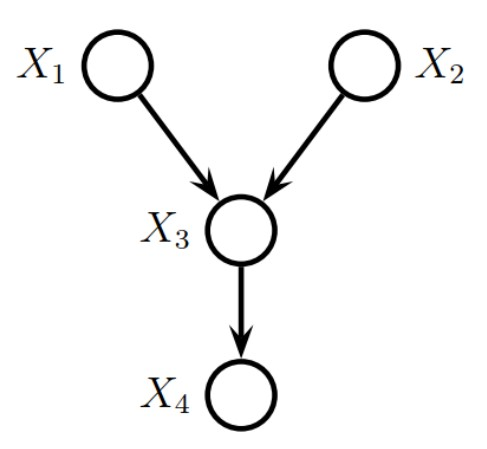
\includegraphics[width=0.45\textwidth]{a2_p11_1}
                \caption{The first graphical model}
            \end{figure}

            Considering the model in Figure 2\ref{fig:m2}, where the random variables that are conditioning on are not shaded because they change based on the problem.
            \begin{figure}[H]
                \label{fig:m2}
                \centering
                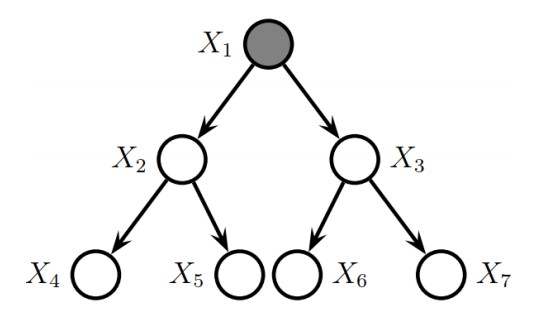
\includegraphics[width=0.5\textwidth]{a2_p11_2}
                \caption{The second graphical model}
            \end{figure}
            \begin{enumerate}[label=(\alph*), resume]
                \item Is $X_4 \perp X_7 | X_1$ ?
                \item Is $X_4 \perp X_5 | X_1$ ?
            \end{enumerate}
        \end{problem}

        \begin{solution}
            
        \end{solution}

        %=================== Problem 2 ===================%
        \begin{problem}
            [Naive Bayes Classifier (NBC)]\\
            Naive Bayes Classifier is widely used to classify emails. It can be expressed as a graphical model as shown in Figure 3\ref{fig:m3}, where $Y$ is the class label, $Y \in \{0, 1\}$. The class 1 means spam email and the class 0 means non-spam email.
            Random varialbes $X$ represent the features of the emails. For instance, $X_A$ can be the number of words in an email, $X_B$ can be the time of day receiving the emails, and $X_C$ can be the number of words not found in dictionary.
            Let us assume that these three features are \textbf{Gaussian distributed}, alrhough this assumption is not entirely accurate. Let us also assume that $Y$ is \textbf{Bernoulli} with $p(Y=1 | \pi) = \pi$
            \begin{figure}[H]
                \label{fig:m3}
                \centering
                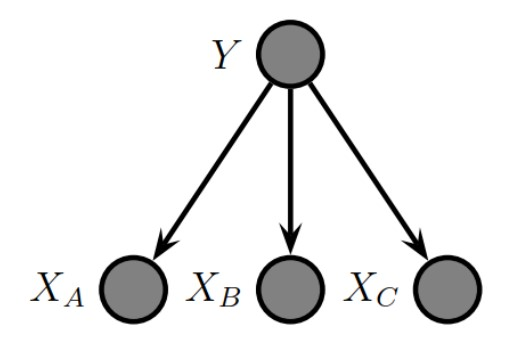
\includegraphics[width=0.5\textwidth]{a2_p12}
                \caption{The NBC graphical model}
            \end{figure}
            \begin{enumerate}[label=(\alph*)]
                \item Write down the joint probability of the random variables in the graph and factorize it according to the graph structure.
                \item For all pairs of features ($X_i$ and $X_j$, $i \neq j$),
                is $X_i \perp X_j | Y$? Explain what this means with respect to the problem of classification and the implications for the features.
                Is this true of our real data in practice?
                Can you think of a situation when this assumption will be explicitly violated, and may impact our classification accuracy? (answer in two sentences)
                \item We have a training set
                      $$
                      D_{training} = \{ (Y, X_A, X_B, X_C)_1, \dots, (Y, X_A, X_B, X_C)_n \}
                      $$
                    (with observed features and class lables, in other words, $n$ emails classified as spam or not spam), and a test set
                      $$
                      D_{test} = \{ (X_A, X_B, X_C)_1, \dots, (X_A, X_B, X_C)_{n+m} \}
                      $$
                    (with oberved features, but unknown class labels).\\
                    With this classifier, we could predict the probability that a test email belongs to the spam class. Write down how to compute $P(Y_j=1 | (X_A, X_B, X_C)_j$, where $j=(n+1), (n+2), \dots (n+m)$; given that we know the components of our factorized joint probability.
            \end{enumerate}
        \end{problem}

        \begin{solution}
            
        \end{solution}

        %=================== Problem 3 ===================%
        \begin{problem}
            [Maximum likelihood estimates for NBC]\\
            Still use the graph in Figure 3\ref{fig:m3} and the task of classifying emails. Let's focus on the training data,
            $$
                D_{training} = \{ (Y, X_A, X_B, X_C)_1, \dots, (Y, X_A, X_B, X_C)_n \}
            $$
            Suppose our features $X_{A,B,C}$ in each class of emails have Gaussian distributions, e.g. $X_A|Y = y \overset{\mathrm{iid}}{\sim} \Gaussian(\mu_{A,y}, \sigma_{A,y}^2)$.
            In other words, the Gaussian parameters for the features are class-specific, meaning that there is one mean for feature $A$ when the email is pam and another mean for feature $A$ when it is not spam.
            \begin{enumerate}[label=(\alph*)]
                \item $Y \overset{\mathrm{iid}}{\sim} Ber(\pi)$, $\pi \in {[0, 1]}$. How do we find the MLE of $\pi$ using the training set $D$?
                \item If $\sigma_{A,y}^2$ is fixed, derive the MLE of $\mu_{A,1}$ and $\mu_{A,0}$ (in other words, the class mean of feature A for spam and not spam) using training set D.
                \item If $\mu_{A,1}$ and $\mu_{A,0}$ are fixed, derive the MLE for $\sigma_{A,0}^2$ using traning set D.
            \end{enumerate}
        \end{problem}

        \begin{solution}
            
        \end{solution}
    \end{section}
    
    \begin{section}{Problem 2}
        \setcounter{pcounter}{0}
        We have studied in class how to construct generalized linear models:
        $$
            \xi = \theta^T x, \mu=f(\xi), \eta=\psi(\mu)
        $$
        %=================== Problem 1 ===================%
        \begin{problem}
            [Poisson Regression]\\
            Under the framework, we want to model the data $\{(x_i, y_i)\}$ using Poisson as the conditional distribtuion of response variables $p(y|x, \lambda) = \frac{\lambda^y e^{-\lambda}}{y!}$.
            \begin{enumerate}[label=(\alph*)]
                \item Find the canonical response function $f(\cdot)$;
                \item Derive the batch gradient descent update rule;
                \item Derive the batch Newton descent update rule;
                \item Derive the strocastic gradient descent update rule.
            \end{enumerate}
        \end{problem}

        \begin{solution}
            
        \end{solution}

        %=================== Problem 2 ===================%
        \begin{problem}
            [Multi-class Logistic Regression]\\
            As we discussed in class, we can also use category distribution GLIM to generalize logistic regression to multi-class classification.
            \begin{enumerate}[label=(\alph*)]
                \item Follow what we discussed in class, write down the MLE using the category distribution GLIM;
                \item Derive the batch gradient descent update rule.
            \end{enumerate}
        \end{problem}

        \begin{solution}
            
        \end{solution}
    \end{section}

    \begin{section}{Problem 3}
        \setcounter{pcounter}{0}
        %=================== Problem 1 ===================%
        \begin{problem}
            [Linear Regression]\\
            Some researchers who are desperately in need of a machine learning expert bring you a dataset with information on $n = 1100$ people.
            Their study has two explanatory predictors: $X_1=a$ binary indicator of gender (female=1 and male=0), and $X_2=$some weight.
            They want to use this information to help predict blood pressure $Y$ which they believe is linearly related to $X_1$ and $X_2$.\\
            Suppose that $\sigma^2 = 1$ and for part (c) $\tau^2=1$. Use the first 1000 records for your training set, and the last 100 records for your test set.
            For this answer, \textbf{include your code (R, Matlab, python, etc.) in your solution}, but please do not use built in functions for linear regression. The dataset is HW2\_linear\_regression.txt.
            \begin{enumerate}[label=(\alph*)]
                \item Write a program to estimate $\beta$ using the \textbf{normal equation}. Estimate $\beta$ from the training set.
                \item Write a program to estimate $\beta$ usign \textbf{stochastic gradient descent}. Estimate $\beta$ from the tranining set.
                \item Write a program to estimate $\beta$ using the \textbf{ridge regression normal eqaution}. Estimate $\beta$ from the training set.
            \end{enumerate}
            For all of the above estimation procedures:
            \begin{enumerate}[resume, label=(\alph*)]
                \item Calculate $RSS(\hat{\beta}) = \frac{1}{n} \sum_{i=1}^{n} (yi - \hat{\beta} x_i)^2$ in the training dataset;
                \item Calculate $RSS(\hat{\beta})$ in the test dataset;
                \item For each of the estimated values of $\hat{\beta}$, what is $E[Y|X=[1,135]^T, \hat{\beta}]$ ?
            \end{enumerate}
        \end{problem}

        \begin{solution}
            
        \end{solution}

        %=================== Problem 2 ===================%
        \begin{problem}
            [Logistic Regression]\\
            The researchers this time are interested in doing prediction for a binary outcome $Z$ (an indicator of adverse reaction to a drug they are testing), which they again beleive is linearly related to $X_1$ and $X_2$.\\
            Again, use the first 1000 records for your training set, and the last 100 records for your test set. The dataset is in n HW2\_logistic\_regression.txt.
            \begin{enumerate}[label=(\alph*)]
                \item Write a program to estimate $\beta$ using the alogrithm introduced in class. Estimate $\beta$ using the training data;
                \item Calculate $RSS(\hat{\beta})$ in the training dataset;
                \item Calculate $RSS(\hat{\beta})$ in the test dataset;
                \item What is $E[Z|X=[1,135]^T, \hat{\beta}]$?
            \end{enumerate}
        \end{problem}

        \begin{solution}
            
        \end{solution}
    \end{section}

\end{document}